\documentclass[aps,pra,reprint,a4paper,nofootinbib,superscriptaddress,numbers,longbibliography,showpacs,showkeys,floatfix]{revtex4-1}
\usepackage{hyperref,color,graphicx}
\usepackage{amsfonts,amssymb,amsmath}
\usepackage[separate-uncertainty=true]{siunitx}

% \usepackage{dblfloatfix}
% \usepackage{stfloats}

\DeclareSIUnit\gauss{G}

\usepackage[english]{babel}
\usepackage[utf8]{inputenc}
\usepackage[T1]{fontenc}
% \usepackage{trace}
\usepackage{bm}
\usepackage{wasysym}

\usepackage{comment}
\usepackage{xspace}

\newcommand{\coloneqq}{\mathrel {\mathop : } \mathrel {\mkern -1.2mu}=}

\usepackage{bbm} 
\newcommand\identity{\ensuremath{\mathbbm{1}}}
	
\DeclareMathOperator{\sinc}{sinc}
\DeclareMathOperator{\module}{mod}

% \def\bra#1{\mathinner{\langle{#1}|}}
% \def\ket#1{\mathinner{|{#1}\rangle}}
% \def\braket#1{\mathinner{\langle{#1}\rangle}}
\def\bra#1{\left\langle#1\right|}
\def\ket#1{\left|#1\right\rangle}
\def\braket#1#2{\left\langle#1\kern-2pt\right.\left|#2\right\rangle}
%
\newif\ifusebibfile
\usebibfiletrue
% \pdfminorversion=7
% \pdfsuppresswarningpagegroup=1

\textheight=1.0\textheight

\newcommand{\figref}[2]{\hyperref[#1]{\ref{#1}(#2)}} % Reference to subfigures.

\newcommand{\encapsulateMath}[1]{\raisebox{0pt}[0pt][0pt]{#1}}

\hypersetup{
 pdftitle = {Attaining the quantum speed limit beyond local coupling with atomic wave packets},
 pdfauthor = {Manolo Rivera Lam, Natalie Peter, Thorsten Groh, Carsten Robens, Wolfgang Alt, Dieter Meschede, Antonio Negretti, Tommaso Calarco, Andrea Alberti},
	colorlinks=true,linkcolor=blue,citecolor=blue,filecolor=blue,urlcolor=blue,pdfpagemode=UseNone,pdfstartview={XYZ null null 1.00}
}

\newcommand{\figlab}[1]{{\textbf{{#1}}}} % Subfigure label in caption.
\newcommand{\vect}[1]{\boldsymbol{#1}} % Vector notation: bold style.
% \newcommand{\vect}[1]{{\vec{{#1}}}} % Vector notation: arrow.
\newcommand{\op}[1]{{{#1}}} % Operator notation: no hat.
% \newcommand{\op}[1]{{\hat{#1}}} % Operator notation: hat
\newcommand{\imag}{{\mathrm{i}}} % imaginary i
\newcommand{\e}{{\mathrm{e}}} % Euler e
% \pdfstringdefDisableCommands{\def\eqref#1{(\ref{#1})}} % Enable eqref in title

\renewcommand\textemdash{\leavevmode\unskip\kern0.8pt\rule[0.19\baselineskip]{8pt}{0.4pt}\kern1pt\ignorespaces}

\newcommand{\MT}{Mandelstam-Tamm\xspace}

\usepackage{editing}

\newchange{Andrea}{DarkBlue}{Orange}

\newnote{Andrea}{purple}

\changeAndreaOn
\noteAndreaOn

\begin{document}

\title{
Delocalizing atomic wave packets at the quantum speed limit\\ %
Controlling atomic wave packets at the quantum speed limit\\ % Andrea, Wolfgang
Observation of quantum speed limit\\
Observation of quantum speed limit by splitting atomic wave packets\\
Observation of quantum speed limit by coherent splitting of atomic wave packets\\
Splitting atomic wave packets at the quantum speed limit\\
Realizing transport of atomic wave packets at the quantum speed limit\\
Realizing optimal transport of atomic wave packets at the quantum speed limit\\ % Antonio
Transporting atomic wave packets at the quantum speed limit % Antonio
}

\title{Attaining the quantum speed limit beyond local coupling with atomic wave packets}

\newcommand{\affA}{Institut f\"ur Angewandte Physik, Universit\"at Bonn, Wegelerstra\ss{}e 8, D-53115 Bonn, Germany}
\newcommand{\affB}{Departement of Physics, Massachusetts Institute of Technology, Cambridge, MA 02139}
\newcommand{\affC}{Zentrum f\"ur Optische Quantentechnologien and The Hamburg Centre for Ultrafast Imaging, Universit\"at Hamburg, Luruper Chaussee 149, D-22761 Hamburg}
\newcommand{\affD}{Forschungszentrum J\"ulich, Wilhelm-Johnen-Straße,
52428 J\"ulich, Germany}


\author{Manolo Rivera Lam}\affiliation{\affA}
\author{Natalie Peter}\affiliation{\affA}
\author{Thorsten Groh}\affiliation{\affA}
\author{Wolfgang Alt}\affiliation{\affA}
\author{Carsten Robens}\affiliation{\affB}
\author{Dieter Meschede}\affiliation{\affA}
\author{Antonio Negretti}\affiliation{\affC}
\author{Tommaso Calarco}\affiliation{\affD}
\author{Andrea Alberti}\affiliation{\affA}
\email{alberti@iap.uni-bonn.de}

\begin{abstract}
Controlling quantum processes faster than the decoherence rate is a fundamental challenge for any technology based on quantum mechanics.
%
% Controlling quantum processes faster than the decoherence rate \textemdash a unavoidable/ubiquitous source of information loss \textemdash is a fundamental challenge for any technology based on quantum mechanics.
%
Ultimately, however, quantum mechanics sets limits on the shortest time required to carry out a quantum process with unit fidelity, which depends on the distance between the initial and final state, and on the energy available to control the process.
%
% There is, however, a minimum time necessary to carry out a given quantum process.
\begin{comment}
, which depends on the distance between the initial and final quantum states, and on the energy available to control the states of the system.


In real systems, however, there is a minimum time required to execute a particular quantum process.

, which is imposed by quantum mechanical laws and by the amount energy available to control the quantum states of the system.

Such a minimum time defines the so-called quantum speed limit for the specific quantum process, below which the system is not quantum controllable, meaning that the chosen quantum process cannot be executed with high fidelity.

Such a minimum time defines the so-called quantum speed limit of the process.

Here, we report on the observation of the quantum speed limit in realizing a single-atom Mach-Zehnder interferometer in position space:
\end{comment}
%
We here demonstrate the existence of such a quantum speed limit by transporting single atoms in optical potentials between sites situated at a distance of 20 times the size of the original wave packet.
%
By splitting and recombining the wavefunction of each atom in a Mach-Zehnder type interferometer, we directly attest the quantum coherence of the fast transport operations.
%
Leveraging quantum optimal control theory, we steer the movable potentials so as to maximize the overlap of the transported wave packet with the ground state wavefunction in the target site.
%
The fidelity of the process measured as a function of the transport duration exhibits a behavior that is believed to be universal.
%
\begin{comment}
: as the transport process becomes faster and faster, the fidelity drops abruptly from unity to zero.

, showing a transition from a quantum controllable process to one that is no longer controllable.
that is controllable to one that cannot be longer controlled.

The quantum speed limit shown here is a limitation of quantum technologies at large, and at the same time demonstrates a single-atom interferometer at the quantum speed limit, a fundamental building block for quantum computing with neutral atoms in optical lattices and
\end{comment}
%
These results are a paradigmatic demonstration of the existence of a quantum speed limit to which quantum technologies are subject, and constitute an important step on the way to quantum computing with neutral atoms in optical lattices.

\begin{comment}
fast atom interferometer demonstrates a fundamental building block for quantum computing with neutral atoms in optical lattices, and holds promise to boost the sensitivity of atom interferometers.

where the single-atom sensitivity can reach its optimum by optimizing the space-time area enclosed by interferometer.


Depending on their electron spin state, trapped Cesium atoms are displaced in space at the highest speed allowed by quantum mechanical laws.

The quantum speed limit describes a fundamental upper bound on how fast a quantum system can evolve. We investigate the maintenance of the motional ground state of neutral atoms in a potential during the transport in a state-dependent coveyer belt. With the numerical solutions of quantum optimal control theory we identify experimentally the quantum speed limit and apply them to an atom interferometer.
We show that the realization of quantum speed limit also holds in a quantum interferometer.
\end{comment}
\end{abstract}

%\date{\today}
\maketitle 


% Quantum computing and related quantum technologies rely on quantum processes to transform information encoded in the quantum states of the system.
%
% During such processes, fragile coherent superposition states are created, which are very vulnerable to noise induced by the environment.
%
% Quantum computing rely on fragile quantum superposition states in order to process information more efficiently than using classical computers.
%
Quantum computers process information more efficiently than classical computers by harnessing the power of quantum superposition states.
%
% Such states are extremely fragile though, as they are vulnerable to noise induced by the environment, which entangles the degrees of freedom of the system with those of the environment.
These states, though, are extremely fragile, as they are vulnerable to environment-induced noise causing their rapid decoherence.
%
% Fortunately, a remedy against decoherence effects exists,
%
% Andrea's comment [2019-10-23 11:13:25]: Todo: choose among these citations \cite{Calderbank:1996,Steane:1996,Steane:1996a,Cory:1998,Chiaverini:2004,Schindler:2011,Reed:2012,Kelly:2015,Linke:2017} 
Fortunately, the detrimental effects caused by decoherence can be cured using
quantum error correction protocols
\cite{Calderbank:1996,Steane:1996a}.
% , which enable the correction of physical errors while leaving the stored quantum information intact.
%
To achieve fault-tolerant quantum computation, however, the fidelity of the individual quantum processes involved in the computation must surpass a minimal threshold level \cite{Knill:1998}, whose value depends on the specific protocol, and is generally believed to lie above \SI{99}{\percent}. Thus, several techniques have been put forward in order to enhance the fidelity of quantum processes, which include
spin-echo pulses \cite{Andersen:2003,Kuhr:2005,Kleine-Buning:2011}, dynamical decoupling \cite{Viola:1998,Fortunato:2002,Fraval:2005,Biercuk:2009,Du:2009,Sagi:2010}, decoherence-free subspaces \cite{Home:2009,Timoney:2011,Wang:2016g}, holonomic quantum gates \cite{Pachos:2001,Duan:2001a}, topological quantum codes \cite{Dennis:2002a}, and fast driving protocols \cite{Campbell:2010,Schaefer:2018}.
%
Among these techniques, fast driving protocols hold center stage,
% appear to play a special role,
for they can be combined with virtually any of the other techniques, and are applicable to all quantum systems.
%
The basic idea behind them is that by outrunning decoherence, one can effectively mitigate its adverse effects.
%
% The basic idea behind this technique is fast driving protocols can outrun decoherence an in order to mitigate its detrimental effects.
%
% The question, thus, arises as to how fast quantum processes can be performed and what determines their \emph{quantum speed limit}.
%
It is thus relevant to determine how fast quantum processes can be performed and what defines their \emph{quantum speed limit}.
%
% Such a question is of great interest not only because of the foregoing quantum-technological implications, but also because of its fundamental character.
%
Moreover, controlling a system at its quantum speed limit is not only relevant for quantum technologies, but also because it helps us better understand fundamental aspects about the evolution of quantum systems.
%
% has become of great interest in recent years, not only because of its fundamental character, but also and more importantly because of its relevance in view quantum technological applications.

% It has long been known in classical physics that there exist a minimum time necessary to carry out a given physical process, at least since Bernoulli's famous brachistochrone problem.
% %
% Such a minimal time exists in quantum physics too, for this is a consequence of the fact that resources are finite, namely that there is a limited amount of energy available to control the process.


It has long been known in classical physics that physical processes require a minimal time to carry out a certain transformation, as exemplified by Bernoulli's famous brachistochrone problem \cite{Haws:1995}.
%
Such a speed limit reflects the fact that the energy available to control any process is ultimately finite.
% \textemdash a condition to which all physical processes are universally subject.
%
% The physical reason of such a speed limit can be traced back to the fact that physical resources are finite, or, more precisely, to the fact that the energy available for controlling the process is limited \textemdash a constraint to which all physical systems are universally subject.
%
By the same token, it is thus natural to expect that an analogous speed limit also applies to quantum processes.
%
Indeed, such a quantum speed limit has been recognized by Mandelstam and Tamm \cite{Mandelstam:1945}, observing that the maximum rate of change of a quantum state is bounded by its energy uncertainty.
 % there is a relation between the energy uncertainty of a given quantum state and its maximal rate of change.
%
In fact, generalizing this result to time-dependent quantum systems, Anandan and Aharonov \cite{Anandan:1990} have derived the following inequality:
%
\begin{equation}
	\label{eq:MT-bound}
	%\tau  = \frac{\hbar \, \mathcal{L}\{\ket{\psi(t)}\}}{\langle\Delta E\rangle} \geq \frac{\hbar \cos^{-1}(|\langle\psi_A|\psi_B\rangle|)}{\langle\Delta E\rangle},
	\frac{\cos^{-1}(\left|\braket{\psi_A}{\psi_B}\right|)}{\tau} \leq \frac{\langle\Delta E\rangle}{\hbar},
	% \tau \geq \frac{\hbar \cos^{-1}(|\langle\psi_A|\psi_B\rangle|)}{\langle\Delta E\rangle},
\end{equation}
where $\tau$ is the duration of a quantum process transforming a quantum state $\ket{\psi_\text{A}} \coloneqq \ket{\psi(0)}$ into $\ket{\psi_\text{B}} \coloneqq \ket{\psi(\tau)}$,
% $\mathcal{L}\{\ket{\psi(t)}\}$ is the arc length in the Hilbert space of the time-evolved quantum state $\ket{\psi(t)}$ computed with Fubini-Study metric \cite{Bengtsson:2017},
$\hbar$ is the reduced Planck constant, and $\langle \Delta E \rangle$ is the time-averaged energy uncertainty derived from the system's Hamiltonian $\hat{H}(t)$ \cite{defDeltaH}.
%
% The inequality in Eq.~(\ref{eq:MT-bound}) simply states the fact that the arc length, $\mathcal{L}\{\ket{\psi(t)}\}$, is always greater than (or equal to) the Fubini-Study distance between the initial and final states, $\cos^{-1}(|\langle\psi_A|\psi_B\rangle|)$;
%
It is important to note that the inverse cosine on the left-hand side of Eq.~(\ref{eq:MT-bound}) represents a measure of how the evolved state differs from the initial one, expressed in terms of the Fubini-Study metric \cite{Bengtsson:2017}.
%
% Several generalizations of the Mandelstam-Tamm bound have later been found for nonunitary processes \cite{Deffner:2017a}, and
%
% Owing to its universal character and its practical implications in quantum technologies, the Mandelstamm-Tamm bound has recently attracted great interest by the scientific physics community \cite{Deffner:2017a}.

test Carsten

Owing to its universal character and its practical implications in quantum technologies, the quantum brachistochrone problem has been the subject of intense research in recent years \cite{Deffner:2017a}.
%
Importantly, it has been realized that the bound in Eq.~(\ref{eq:MT-bound}), generally known as Mandelstam-Tamm bound, can only be saturated in simple two-level systems \cite{Uhlmann:2009}, where the initial and final states are directly coupled to each other through Rabi oscillations.
%
Otherwise, the \MT bound (with its generalizations \cite{Margolus:1998}) can only be attained asymptotically \cite{Levitin:2009} as the system's dynamics reduces to that of two quantum states.
%
Experimentally, the \MT bound was verified in effectively two-level setups based on ultracold atoms \cite{Bason:2012} and superconducting transmon circuits \cite{Vepsalainen:2019}.
%
Recently, however, the notion of quantum brachistochrone as defined based on \MT has 
% as defined in terms of the Mandelstam-Tamm bound,
% as defined based on the Mandelstam-Tamm bound,
been subject to criticism \cite{Bukov:2019}:
%
It has in fact been noticed that in the majority of complex physical systems, where only local couplings between states are accessible, direct Rabi coupling as required to saturate the \MT bound cannot be physically implemented, unless the two states involved are already locally connected.
%
In these systems, the \MT bound fails to capture the true quantum speed limit.
%
% In fact, any useful quantum hardware necessary involves quantum manipulations that go far beyond a direct Rabi coupling between two locally connected states.
%
% In the majority of quantum systems, instead, only local couplings are  physically realizable, which thus excludes the possibility to directly couple states that are nonlocally connected.
%
% For these complex systems, the bound in Eq.~(\ref{eq:MT-bound}) fails to capture the true quantum speed limit.
%
In this work, we give the first experimental demonstration of quantum control of a physical system at its quantum speed limit, where the initial and final states are not locally connected.
%
Specifically, we consider the problem of transporting an atomic matter wave from the motional ground state of an initial site A to the motional ground state of a site B, where A and B are not locally connected, as they are situated at a distance of about 20 times the size of the initial wave packet; see Fig.~[\figref{Fig:Transport_Ramp}{a}].
%
Naturally, our experimental apparatus only involves local couplings between states, as we steer the atomic wave packets by controlling the trapping potential, precisely its position and depth.
%
The trap depth, in addition, is constrained not to exceed a maximum value, as this reflects the universal fact that the energy available for quantum process control is ultimately limited.
%
% This generally applies to any trapping potential, whose depth is necessarily finite, and reflects the universal fact that the energy available to control a quantum process is ultimately limited.
%

Fast, high-fidelity transport of atomic matter waves has direct practical interest for the development of quantum technologies \cite{Kielpinski:2002}, and has been investigated by ultracold atoms and trapped ion experiments  \cite{Couvert:2008,Bowler:2012,Walther:2012,Alonso:2016,Ness:2018}.
%These experiments were conducted under the assumption that the trapping potential can be approximated by a harmonic potential \cite{Murphy:2009a,Chen:2010d}.
These experiments have been hitherto conducted assuming that the trapping potential can be approximated by a harmonic potential \cite{Murphy:2009a,Chen:2010d}.
%
Under this assumption, however, the true quantum speed limit of the system cannot be reached, since no speed limit exists for an infinitely extended harmonic potential.
%
In our work, we go beyond the harmonic potential paradigm and make use of full quantum optimal control theory to reach the quantum speed limit of our anharmonic trapping potential, so as to study the transition of our system from a quantum controllable towards a quantum noncontrollable system.



\vspace{1cm}
\noindent{}\textsc{until here}\\[-2mm]
\noindent\rule{\columnwidth}{0.4pt}
\vspace{2mm}


To be cited: \cite{Kaufmann:2018} for preserving quantum information during transport. Quantum computing with neutral atoms \cite{Weiss:2017}.

Also to be cited \cite{Bukov:2019} for QSL along geometric path, and \cite{Anandan:1990} for geometric interpretation of QSL. 

Experimentally: cite paper by D.G.Odelin, Wineland, Schmidkaler, and also J.Sherson \cite{Sorensen:2016a}.



These transformations must be performed with high fidelity, because this allows quantum error correction to be put in place.
%
There is in fact a threshold to the fidelity, below which corrections can be applied repeatedly.



\vspace{3mm}

Keywords:

General introduction:

- Importance of quantum technologies, which requires complex transformation of states including both internal and external degrees of freedom. Here it is important to reach high fidelity.


- State what our definition of quantum speed limit is (which is inspired by relevant quantum technologies). Explain that this definition is compatible with the one assumed by most of scientific literature. 
- Explain the idea of a S-like transition between quantum controllable and non controllable system, stressing that this is a rather universal behavior.

System:

- We control a nontrivial Hilbert space with quantum optical control, involving 10 motional states.
- We show quantum application of this concept controlling both internal and external degrees of freedom (spin-dependent optical lattices play an important role for that)
- Beyond adiabatic concept, we aim at reaching high fidelity in the minimal time allowed by Schrödinger equation.


- Define basic problem of transport, introducing atomic potentials for both spin states. Refer to Fig.1(a) which exemplifies the problem for one spin species.
- Explain that fast transport is possible only through a highly wiggling ramp, far away from the adiabatic limit. Fig.1(b)
- Show that this is indeed realized experimentally in our system, where we need to overcome the problem of the limited bandwidth. We do it by deconvolving the theoretical ramp with the response function of the system.
- Insight about the shape of the ramp, explaining for example why at the beginning the ramp is steeper.
- Mentioning that this fast transport creates many excitations and explores a large Hilbert space, Fig. 1(c).


Experimental apparatus:




List of questions:

- How does it look like the fidelity for highly excited states. Can one optimize transport for both ground state and first excited state?
- What is the best fidelity in transport? Either measure or estimate from current measurements.

\section{Introduction}

\begin{itemize}
    \item In the past decades has been a tremendous experimental and theoretical progress towards coherent control of quantum technologies such as atomic clocks, quantum communications and quantum signal processing.
    \item Powerful methods has been discovered to overcome the problem of decoherence such as quantum error correcting codes~\cite{Kitaev:1997} or identifying shortcuts~\cite{Bason:2012, Chen:2010d} and decoherence-free subspaces.
    \item All processes gain from fast processes and robust control. Besides combating decoherence, quantum computer architectures also gain by speeding up quantum information protocols~\cite{Van-Meter:2013, Kielpinski:2002, Monroe:2013, Weitenberg:2011a}.
    \item Two major challenges of high-speed operations are to overcome technical limitations in order to reach an extremely high degree of quantum control and to determine and realize optimal solutions for systems with many-degrees of freedom.
    
 %In the perspective of quantum computing architecture it remains a challenge to optimize the clock speed towards the fundamental quantum speed limit~\cite{Mandelstam1945, Margolus1998, Taddei2013, Brouzos2015} by improving shuttling and gate operations.
\end{itemize}
 
Brief introduction of our system: 
\begin{itemize}
    \item In previous work, we have demonstrated fast, high-precision transport of cesium atoms in two state-dependent optical lattices~\cite{Robens:2018} and ... (gives some nice applications of our previous results). 
    \item Here, we report the realization of optimal transport by means of optimal control theory under the condition to preserve the motional ground state and identify the quantum speed limit as a sudden decrease of the transport fidelity in good agreement with the numerical and analytical expectation. 
\end{itemize}


Detailed explanation of our setup:
\begin{itemize}
    \item describing our system in more details ~\cite{Karski:2009a} and give some recent results. We do  ultra-fast, optimal control transport across the quantum speed limit of a cesium atom in an optical lattice over one lattice site as shown in Fig. \ref{Fig:Transport_Ramp} a) while maintaining the ground state after the process.
    \item then I want to describe the control parameters and its realization in the system: depth~$U_0(t)$, phase~$\varphi(t)$
        \begin{equation}
        \hat{H}  = \frac{\hat{p}^2}{2m} + U_0(t) \cos^2(k\hat{x} - \varphi(t)/2), 
        \label{eq:Hamiltonian}
        \end{equation}
        
        \begin{equation}
        \hat{U}_{\text{evo}}(T) =  e^{- \frac{i}{\hbar} \int_{0}^{T} \! \hat{H}(t') dt'}
        \end{equation} 
    \item and give a description of its experimental realization with phase and amplitude ramps~Fig.~\ref{Fig:Transport_Ramp} b) and our challenges. There I want to mention that it is difficult to realize ramps on such short time scales (impulse response, deconvolution, ...). Another challenge is how to measure the transport fidelity. Here we present our measurement protocol from Belmechri~\cite{Belmechri:2013}), Fig.~\ref{Fig:BelmechriTechnique}~a), to determine the fidelity directly (MW sideband cooling with 99$\,\%$~efficiency~\cite{Robens:2018}
    \item the we discuss the measurement result, Fig.~\ref{Fig:BelmechriTechnique}~b). The challenge is the number of repetitions vs. decoherence. 
    \item Then I describe the major challenge how to find transport ramps, since there exists no analytic solution for a transport ramp. We approach the QSL numerically by using optimal control theory \cite{Treutlein:2006, Buecker:2011, Rosi:2013}
    \item then I describe how we get optimal control solutions from simulation (cost function, discrete parametrization, ...) 
        \begin{equation}
        \mathcal{F} = |\bra{\psi_{\text{target}}} \hat{U}_{\text{evo}}(T) \ket{\psi_{\text{init}}} |^2
        \end{equation}
        
        \begin{equation}
        \begin{aligned}
        U(t)       & = U_0 & + & \sum_{m=0}^{M} a_m \sin(\nu_m t) , \quad t \in [0,T]\quad,\\
        \varphi(t) & = \frac{2 \pi}{T} t & + & \sum_{m=0}^{M} b_m \sin(\nu_m t) , \quad t \in [0,T]\quad.
        \end{aligned}
        \label{Fourier_Series}
        \end{equation}
\end{itemize}

%
% SECTION
%

\section*{Results}

The first paragraph discuss the result of the linear and quantum speed limit measurement. In detail:
\begin{itemize}
    \item then discuss the measurement linear transport vs. optimal control, Fig.~\ref{Fig:QSL_measurement}~a). Linear transport was used by many other groups to speed up their transport, but we can do it better. The measurement with optimal control solution~Fig.~\ref{Fig:QSL_measurement}~b) demonstrates a significant improvement and we can identify the quantum speed limit as a sharp border. 
    \item The data is well explained by our theoretical model, which is sensitive to the finite radial temperature as the only free parameter = thermometer
    \item in related work they have shown a single measurement close to the expected quantum speed limit with Bose-Einstein condensates~\cite{Frank:2016, Bason:2012}. 
    \item Linear transport in the non-adiabatic regime has been demonstrated in previous work to speed up transport operations with ions~\cite{Walther:2012, Bowler:2012, Kaufmann:2017a} and neutral atoms~\cite{Couvert:2008, Chen:2010d}.
    \item In addition discuss the analytic solution of the QSL, which scales with inverse of the trap frequency (formula)
    \item then discuss the fact, that the classical speed limit has the same scaling
        \begin{equation}
        \begin{aligned}
        \tau^{\text{classical}} = \sqrt{\frac{2 \, d \, m \, \lambda}{\pi \, U_0}}.
        \end{aligned}      
        \end{equation}
\end{itemize}

The second paragraph describes the interferometer as a nice application. In detail:
\begin{itemize}
    \item first describe an atom interferometer~\cite{Steffen:2012}~Fig.~\ref{Fig:Interferometer}~a), measurement of Ramsey fringe contrast, our challenge is the cross talk of the lattices, which we have to compensate
    \item discuss measurement result~Fig.~\ref{Fig:Interferometer}~b), when using the interferometer at the QSL
\end{itemize}


\section*{Conclusion and Outlook}
\begin{itemize}
     \item Then I want to describe the source of the QSL, the Heisenberg's uncertainty relation for energy and time~\cite{Deffner:2017a, Anandan:1990} % Lloyd:2000,
    \item There exist few papers of state-of-the-art experiments measuring close to the quantum speed limit, which I want to cite~\cite{Frank:2016, Bason:2012}
    \item one sentence conclusion, importance for all experiments, which suffer from decoherences (examples)
    \item outlook: macroscopically separated quantum superpositions on the millimeter scale for interferometry, quantum walks~\cite{Groh:2016}, sensing of external forces, molecule formation~\cite{Liu:2018}, but also for fundamental tests of quantum mechanics such as proving bosonic versus fermionic statistics~\cite{Roos:2017}
\end{itemize}

% Andrea's comment [2019-12-17 13:52:56]: Change label from µs to trapping period
% Andrea's comment [2019-11-26 10:40:55]: Using the formula sqrt(PlanckConstantReduced * 866e-9/sqrt(Cs133Mass*25e-6*BoltzmannConstant))/(2*2^(1/4)*sqrt(pi))*1e9 we find that the width of the wave packet is about 24nm, that is, 18 times shorter than the lattice constant of 433nm. This coincides with the scaling in the figure, where using Illustrator we find the width 17.036/0.979 = 17.4 times shorter than the lattice constant.
\begin{figure*}
	\centering
	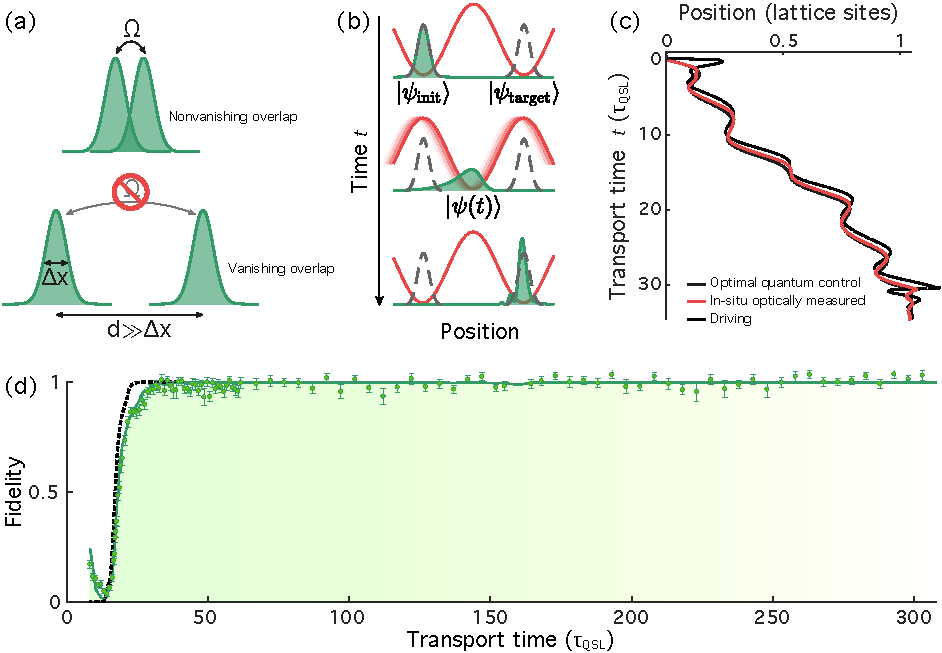
\includegraphics[width=\textwidth]{figure1}
	\caption[]{Scheme of atom transport in an optical lattice (red): a) shows the probability distribution~$\ket{\psi(t)}$ of an atom (green) transported over one lattice site. The fidelity to transfer the atom from the initial to the final motional ground state in a sinusoidal potential is 50$\,\%$. b) compares the optimal control solution with a linear and adiabatic phase ramp in order to reach a transport fidelity of 99$\%$ in the shortest possible duration~$T$ for a constant trap depth~$U_0 = 25\,k_{\text{B}}\, \mu$K.}
	\label{Fig:Transport_Ramp}
\end{figure*}
 
% Andrea's comment [2019-12-17 14:50:01]: We should use Thorsten's figure on p. 41.
% Andrea's comment [2019-12-17 14:52:14]: We should use the shading on top and not below
%
% TODO: Check that the potential corresponds to 25 µk as in Fig.1. Otherwise, what is this potential? Are the wave functions up to scale? Here only 4 states are bound. What potential depth is that? If this is not up to scale, we should simply say it.
% TODO: For Manolo, could you give more details about trap depth and condition for this technique (also duration etc.)
\begin{figure*}
	\centering
	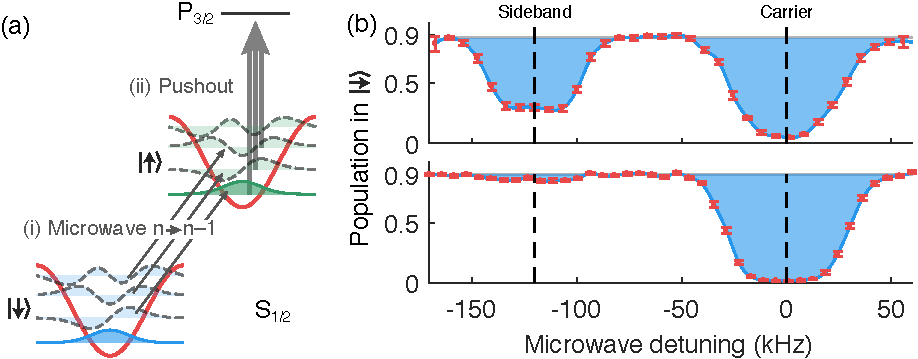
\includegraphics[width=\textwidth]{figure2}
	\caption[]{Precision measurement of ground state occupation. Avoid filling of non occupied motional state in the lower potential.}
	\label{Fig:BelmechriTechnique}
\end{figure*}

% Andrea's comment [2019-12-17 15:23:06]: Carsten suggests to reduce to 150 µs
% Andrea's comment [2019-12-17 15:23:28]: Show time in units of harmonic period
% Andrea's comment [2019-12-17 14:20:28]: Remove from (b) the experimental data of (a).
\begin{figure*}
	\centering
	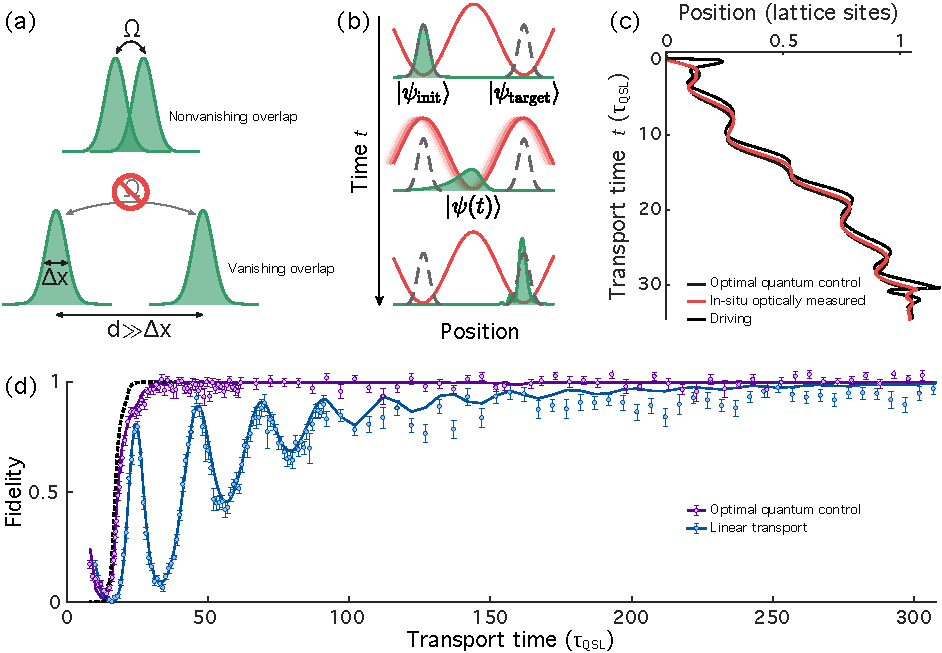
\includegraphics[width=\textwidth]{figure3}
	\caption[]{Measurement of the quantum speed limit (red): a) The fidelity for optimal control solutions suddenly reduces below a certain transport duration, which is identified as the quantum speed limit and shows as a significant improvement in comparison to linear driving ramps (purple). The result is verified by the theoretical expectation for a finite radial temperature (blue) and is even further decreased for a three-dimensional ground state (black).}
	\label{Fig:QSL_measurement}
\end{figure*}
% express x axis in units of trapping frequency
\begin{figure*}
	\centering
	\includegraphics[width=\textwidth]{figure4}
	\caption[]{Interferometer: a) shows the Ramsey fringe contrast (green) of an atom interferometer by applying the ramps, which improves with the transport fidelity. b) The interferometer operates by spatially delocalizing an atom in a superposition of two states (blue and red colored circle) and a coherent recombination. The black lines describe the movement of the two state-dependent lattices.}
	\label{Fig:Interferometer}
\end{figure*}

\bibliographystyle{apsrev4-1}
\bibliography{LiteratureQSL}

\end{document}
